\documentclass{article}
\usepackage[utf8]{inputenc}
\usepackage{authblk}
\usepackage{subcaption} 
\usepackage{natbib}
\usepackage{hyperref}
\usepackage{graphicx}
\usepackage{mathtools}                 % http://ctan.org/pkg/mathtools
\usepackage{amsmath}
\usepackage{listings}
\usepackage[a4paper, portrait, margin=1in]{geometry}
\usepackage[table]{xcolor}
\rowcolors{2}{gray!15}{white}
\newcommand{\head}[1]{%
\textcolor{white}{\textbf{#1}}}
\renewcommand{\arraystretch}{1.5}
\title{\textbf{General Truss Solver}}
\author{Aakash Yadav\\ Email: \href{mailto:me16b001@iittp.ac.in}{me16b001@iittp.ac.in}}
\affil{\textbf{Indian Institute of Technology Tirupati}}
\date{\textbf{May 2019}}
\geometry{a4paper, portrait, margin=1in}

\begin{document}
\maketitle

\begin{center}
\line(1,0){250}
\end{center}


\section{Introduction}
% literature review regarding the usage of this problem
A Truss is an important structure type in structural engineering. A Truss is a essentially a triangulated system of members that are structured and connected in a way such that they only incur axial force. These members are considered two-force members as the forces are only applied at either end of the member, resulting in either a compression or tension force. They are commonly used as bridge designs, given their ability to efficiently span long distances (Refer figure 1). 

In this work, we shall restrain ourselves to planner trusses. A planar truss is one where all members and nodes lie within a two-dimensional plane. The same idea can be extended for solving space trusses i.e. 3D trusses. 
This problem is solved using an in-house Python code developed by the author (\href{https://github.com/AakashSYadav/TrussSolver}{https://github.com/AakashSYadav/TrussSolver}), which solves both deflections and the reactions at the nodes using the Finite Element Method (FEM) approach \citep{jnreddy}.

\begin{figure}[h!]
\centering
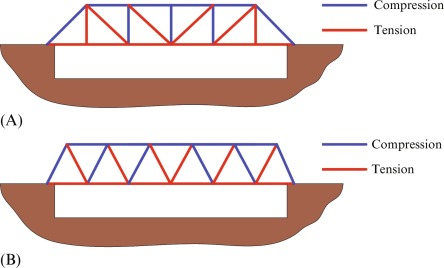
\includegraphics[scale=.6]{3.jpg}

\label{fig:fig1}
\end{figure}
\begin{figure}[h!]
\centering
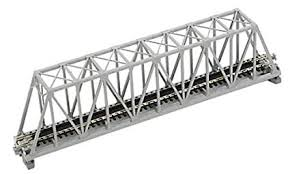
\includegraphics[scale=.6]{4.jpeg}
\caption{Common applications of Truss structures}
\label{fig:fig1}
\end{figure}

In section 2, we bring equtions governing the truss, form the required matrix form and solve a sample problem manually by hand. The section will provide insights to boundary conditions at the nodes. The problem solved manually in section 2 can be used as an template forming the generic/softcoded algorithm in section 3. In section 4, we present the results obtained using the inhouse code and  compare them with the manual solution. In the final section we present the conclusions. All the algorithms implemented in this work can be found in the appendix (or Attachment).

\section{Sample problem and its Manual Solution}

We consider a two-element truss problem as shown in Fig. 2, with the nodes being assigned arbitrary “global” numbers from 1 to 3. Since each node can in general move in two directions, there are $3 \times 2 = 6$ total degrees of freedom in the problem. The global stiffness matrix will then be a $6 \times 6$ array relating the six displacements to the six externally applied forces. Only one of the displacements is unknown in this case, since all but the vertical displacement of node 2 (degree of freedom number 4) is constrained to be zero. Figure 3 shows the global numbers, and also “local” numbers for each individual element. Using the local numbers, the $4\times4$ element stiffness matrix of each of the two elements can be evaluated according to equation shown in figure 4, where $c=cos\theta$ and $s = sin\theta$

\begin{equation}
\theta = \arctan\left(\frac{y_2-y_1}{x_2-x_1}\right)
\end{equation}
Here $x_1, x_2, y_1, y_2$ are the local node numbers for the truss element.
\begin{figure}[h!]
\centering
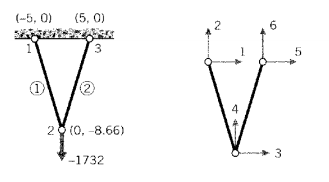
\includegraphics[scale=.7]{1.png}
\caption{A two membered truss with global nodes}
\label{fig:fig1}
\end{figure}

\begin{figure}[h!]
\centering
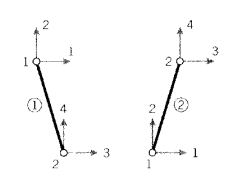
\includegraphics[scale=.7]{2.png}
\caption{Local nodes for the problem in fig 2}
\label{fig:fig2}
\end{figure}

\begin{figure}[h!]
\centering
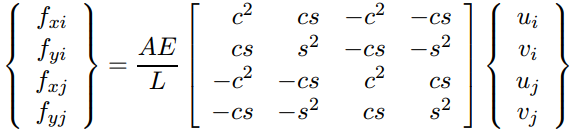
\includegraphics[scale=.5]{5.png}
\caption{Equation for the element truss in global coordinates}
\label{fig:fig2}
\end{figure}

Using the equation shown in fiqure 4 we can write the global $k$ matrices (ref fig 5) for the truss elements. We can use the equation 1 to find the angle for each truss element. For the given problem we have rigidity  modulus of both elements as $E = 10 Mpsi$ and both have area, $A = 0.1 in^2$.

\begin{figure}[h!]
\centering
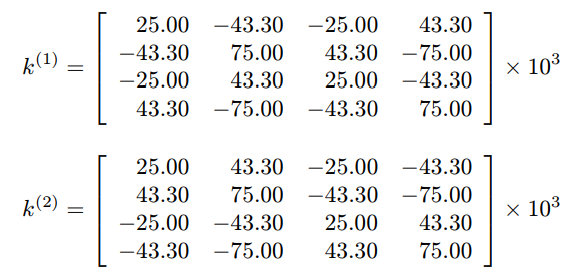
\includegraphics[scale=.6]{6.png}
\caption{Global stiffness matrix for truss elements}
\label{fig:fig1}
\end{figure}

Each of the local degrees of freedom for the truss elements can be matched to one of the global degrees of the overall problem and we can form the connectivity matrix (ref fig 6) which can be used for forming the assembled matrix.
\begin{figure}[h!]
\centering
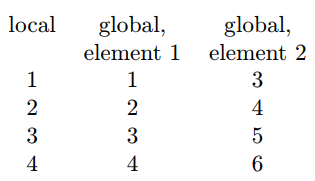
\includegraphics[scale=.6]{7.png}
\caption{Connectivity matrix}
\label{fig:fig1}
\end{figure}
  
Using the connectivity matrix we can write the assembled stiffness matrix as shown in figure 7.
\begin{figure}[h!]
\centering
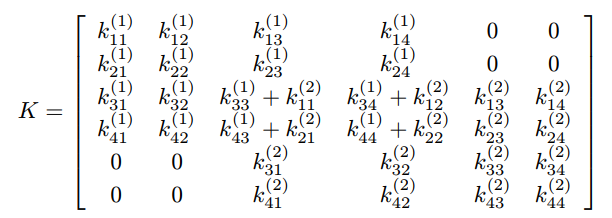
\includegraphics[scale=.6]{8.png}
\caption{Assembly of element matrices}
\label{fig:fig1}
\end{figure}

Fig 8 shows the final system, it can be solved for $u_4$ as $u_4= -0.01155 in$ .
\begin{figure}[h!]
\centering
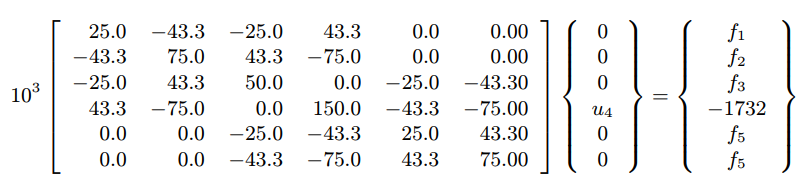
\includegraphics[scale=.6]{9.png}
\caption{Matrix equation obtained by using the assembly}
\label{fig:fig1}
\end{figure}

\section{Methodology and Algorithm}
In this section we provide the algorithms which have been used for solving this problem. 
\begin{table}[ht]
   \centering
   \sffamily
   \begin{tabular}{rlr}
     \rowcolor{black!75}
      \head{No.}& \head{Steps}  \\
     1 & Get the nodes of each element truss from the user        \\
     2 & Calculate angle and length of the trusses \\
     3 & Find the inque number of nodes\\
     4 & Calculate the global k matrices for the elements \\
     5 & Form the connectivity matrix \\
     6 & Assemble the matrices using the connectivity matrices      \\
     7 & Find the unknown parameters  \\
  \end{tabular}
  \caption{Algorithm}
\end{table}


\section{Results}
In this final section we present the results. The results obtained by the program are shown below.
\begin{figure}[h!]
\centering
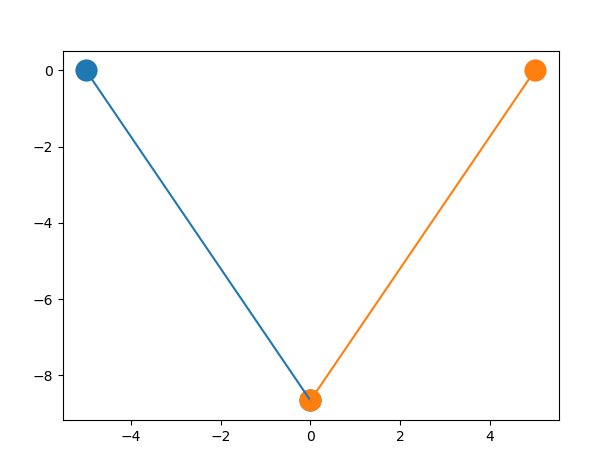
\includegraphics[scale=.6]{10.png}
\caption{Figure showing the geometry generated by the program}
\label{fig:fig1}
\end{figure}

\begin{figure}[h!]
\centering
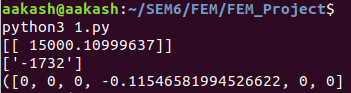
\includegraphics[scale=.6]{11.png}
\caption{Result obtained by the program}
\label{fig:fig1}
\end{figure}


\section{Discussion}
The results obtained by both the methods are inline with each other, hence we can conclude the validation of the code. There have been an active research in this area to optimze the algorithm and speed up the solution procedure citep{Cheng1995} 
\citep{He_2017} \citep{Wei}.



\bibliographystyle{plain}
\bibliography{references}
\end{document}

